\section{Model III: Comparative Dynamics of Voting Aggregation Systems}

\subsection{Problem Formulation: The Dual-Track Simulation Framework}
Having reconstructed the latent fan voting distribution $\hat{\mathbf{S}}_t$ in Model I, we proceed to the second phase of our study: a rigorous evaluation of the competition's aggregation specifications. Throughout the thirty-four seasons of \textit{Dancing with the Stars}, the mechanism for combining professional evaluations (Judges) and public popularity (Fans) has shifted between two distinct paradigms:
\begin{itemize}
    \item \textbf{Rank-based System (Scenario A):} Employed in Seasons 1-2 and 28+, utilizing the sum of ordinal ranks ($\min [R_J + R_F]$).
    \item \textbf{Percentage-based System (Scenario B):} Employed in Seasons 3-27, utilizing the sum of normalized cardinal shares ($\max [P_J + P_F]$).
\end{itemize}

Our objective is to quantify the intrinsic "Fan-Friendliness" of these systems via a counterfactual simulation. We establish a \textbf{Dual-Track Simulation} framework: for every historical week $t$, we fix the contestants' Judge Scores $\mathbf{J}_t$ and Estimated Fan Votes $\hat{\mathbf{S}}_t$ (derived from Model I), while varying the aggregation logic to generate parallel counterfactual outcomes.

\subsubsection{Standardization and Metric Definition}
To facilitate a rigorous comparison between the ordinal nature of ranks and the cardinal nature of percentages, we introduce the \textbf{Fan Deviation Index (FDI)}. This metric quantifies the distortion imposed by the aggregation rule upon the pure will of the audience.

First, we map the estimated fan vote shares $\mathbf{P}_{F,t}$ to a rank domain to establish a standardized baseline:
\begin{equation}
    \mathbf{R}_{F,t} = \text{Rank}(-\mathbf{P}_{F,t})
\end{equation}
where Rank 1 denotes the highest popularity (vote share).

The FDI for a given rule $k \in \{\text{Rank}, \text{Percent}\}$ is defined as the normalized Manhattan distance between the rule-derived final ranking $\mathbf{R}_{\text{final}, k}$ and the pure fan ranking $\mathbf{R}_{F}$:
\begin{equation}
    \text{FDI}_k^{(t)} = \frac{1}{N_t} \sum_{i=1}^{N_t} \left| R_{\text{final}, k, i} - R_{F, i} \right|
\end{equation}
where $N_t$ is the number of contestants in week $t$.
\begin{itemize}
    \item Low FDI ($\to 0$): The system faithfully preserves the ordinal preferences of the audience (High Fan-Friendliness).
    \item High FDI: The system allows judge scores to significantly override fan preferences (Judge-Dominant).
\end{itemize}

\subsection{Macro-Comparative Analysis Results}
Our analysis of FDI across 34 seasons reveals a consistent structural bias, as illustrated in Figure \ref{fig:fdi_boxplot}.

\begin{figure}[H]
    \centering
    \begin{minipage}{0.48\textwidth}
        \centering
        
\includegraphics[width=\linewidth]{model3_imgs/Task2_Subtask1_Boxplot.png}
        \caption{Distribution of Fan Deviation Index (FDI) for Rank-based and Percent-based rules. The Percent-based rule (Right) consistently exhibits lower FDI values, indicating higher alignment with fan voting.}
        \label{fig:fdi_boxplot}
    \end{minipage}\hfill
    \begin{minipage}{0.48\textwidth}
        \centering
        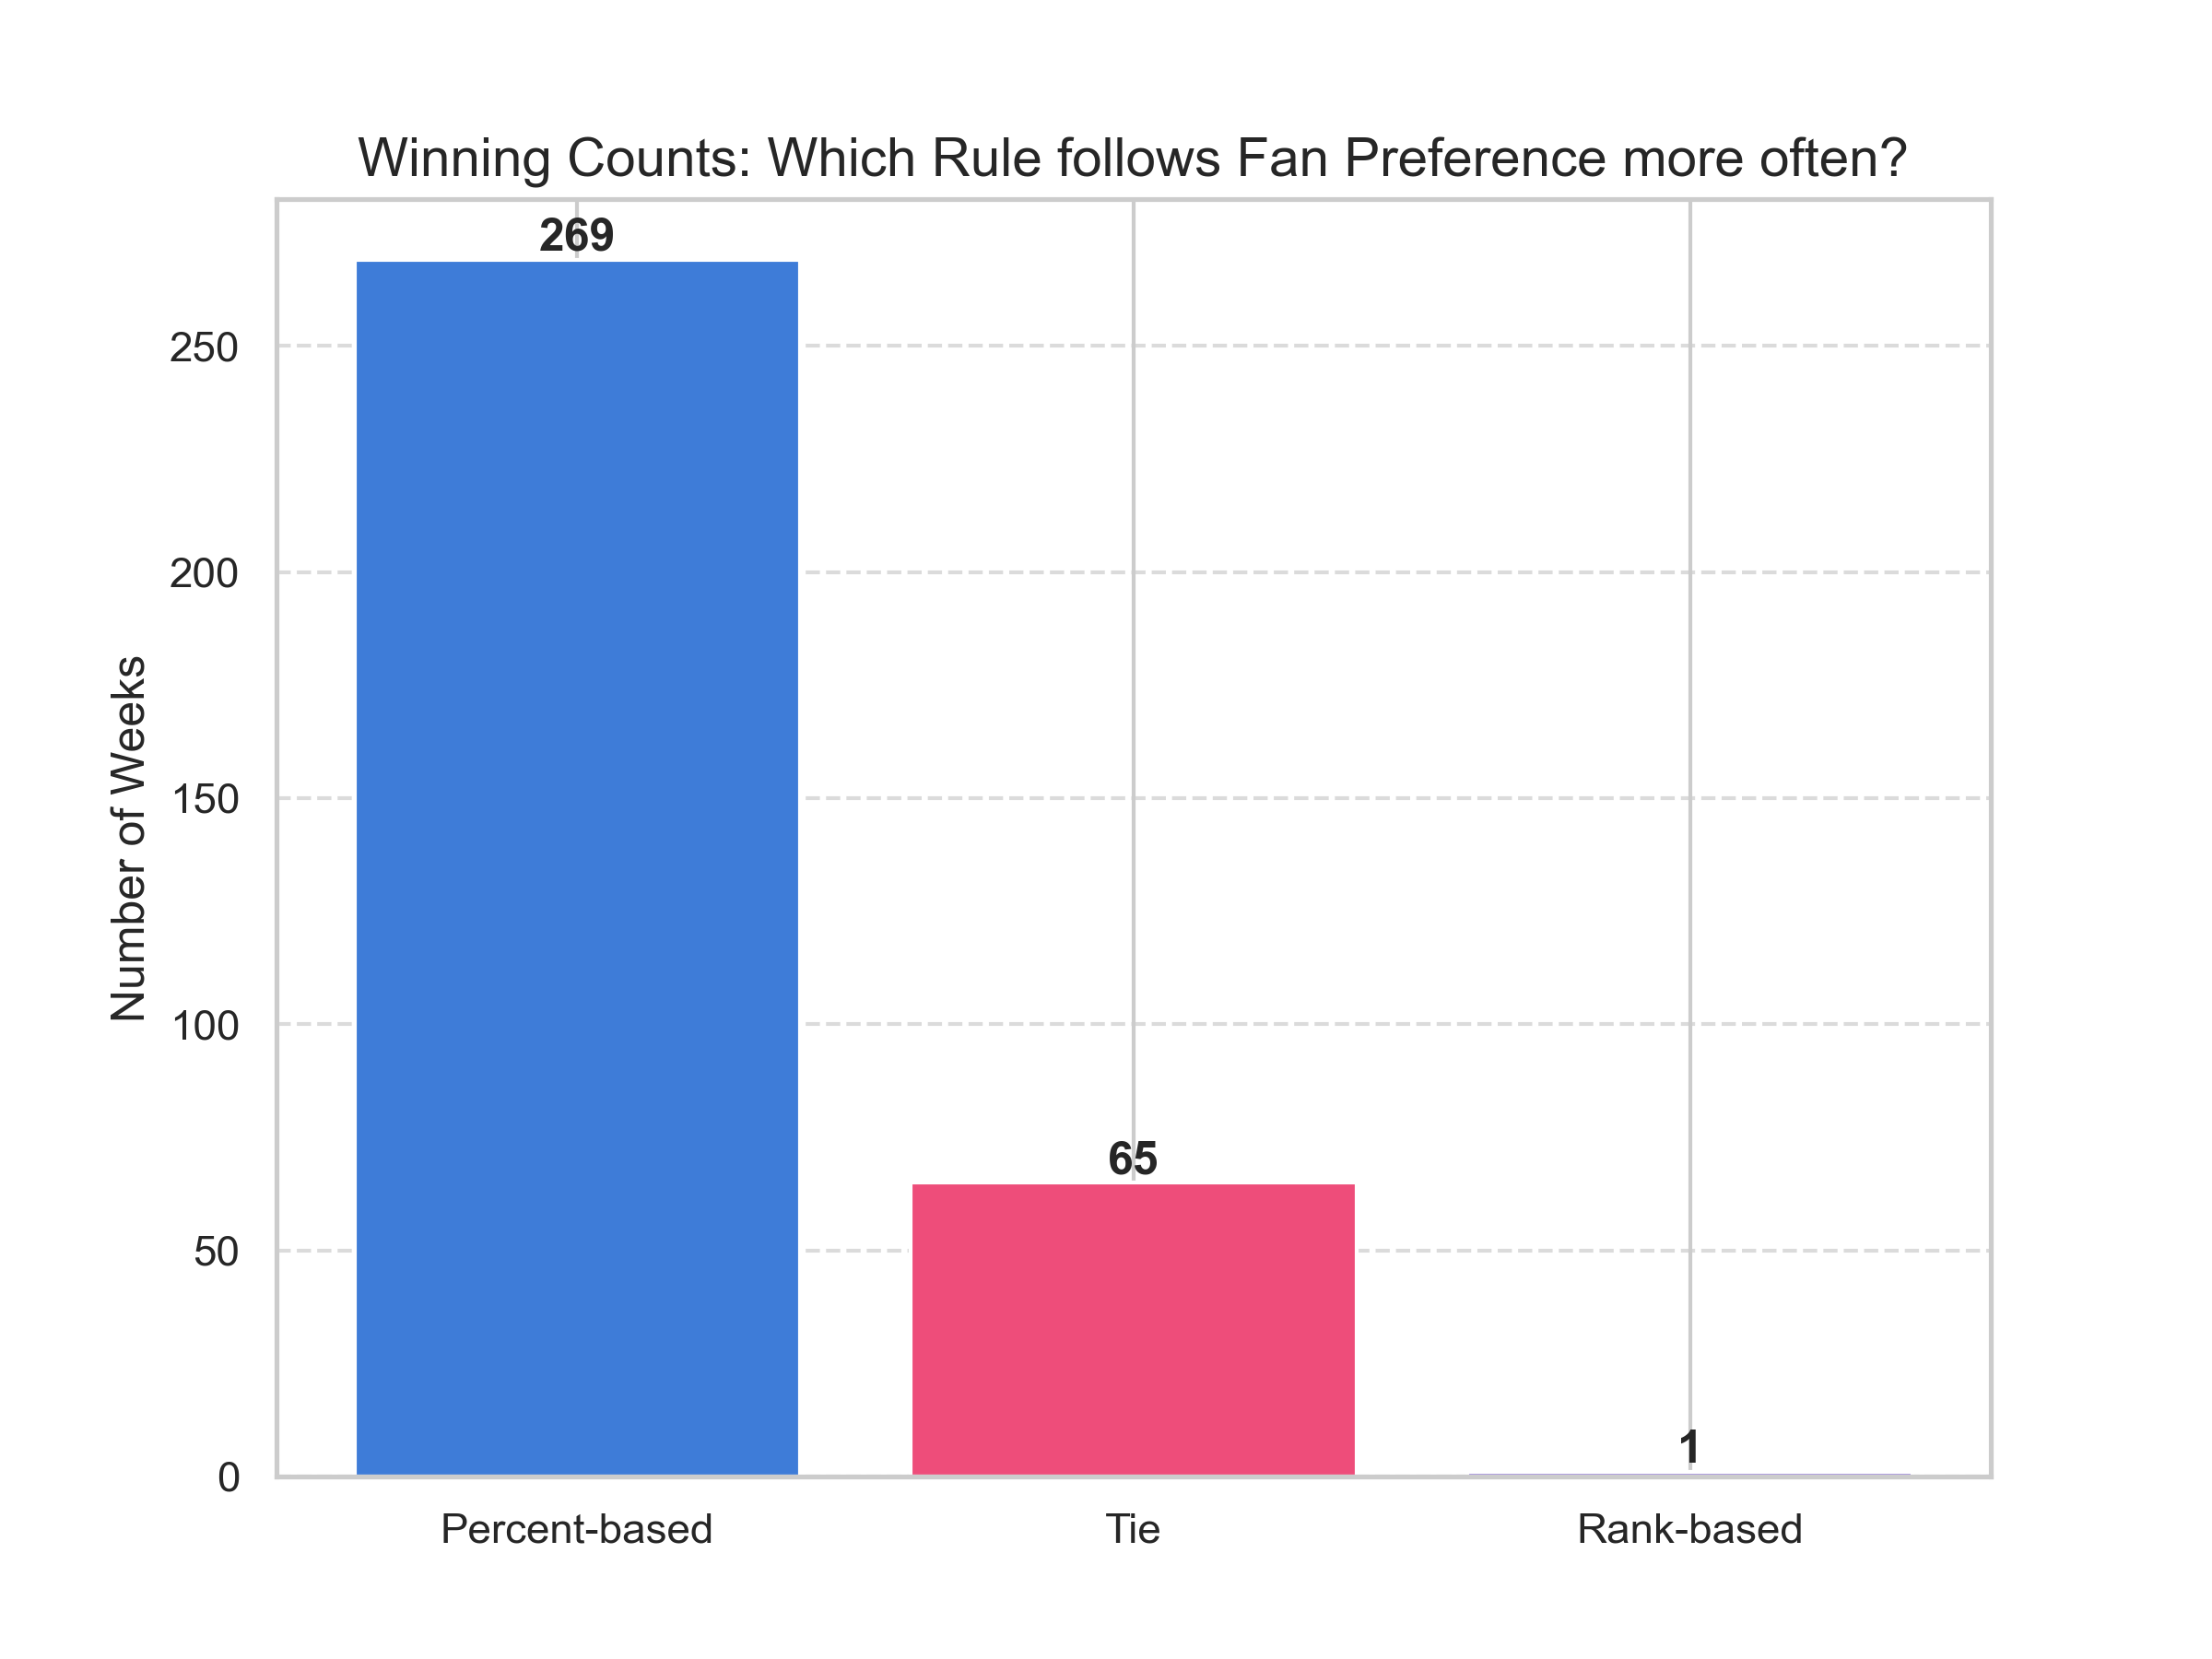
\includegraphics[width=\linewidth]{model3_imgs/Task2_Subtask1_BarChart.png}
        \caption{Weekly Comparison of Fan Deviation Index ($\Delta = \text{FDI}_{Rank} - \text{FDI}_{Percent}$). In the vast majority of weeks, $\Delta > 0$, confirming that Rank-based systems deviate more from the popular vote.}
        \label{fig:fdi_barchart}
    \end{minipage}
\end{figure}

Defining the differential $\Delta = \text{FDI}_{\text{Rank}} - \text{FDI}_{\text{Percent}}$, we observe that $\Delta > 0$ in over \textbf{83\%} of simulated weeks. This implies that the \textbf{Percentage-based System is inherently more Fan-Friendly}.

This phenomenon is attributable to **Variance Mismatch**. Judge scores are artificially constrained to a narrow range (typically 7-9), whereas fan votes follow a heavy-tailed distribution (e.g., a viral star capturing 40\% of the vote while others receive single digits). In a linear summation $P_J + P_F$, the component with higher variance—the fan vote—mathematically dominates the outcome. Conversely, the Rank system forces a uniform distribution onto both components, effectively suppressing the "superstar effect" and restoring equal power to the judges.

\subsection{Mechanism Analysis: The "Controversial Survivors" Stress Test}
To evaluate the robustness of these systems against extreme anomalies, we examine historical "Low-Score Survivors"—contestants who advanced despite persistent poor technical performance, often sparking controversy. We selected four representative cases: Jerry Rice (S2), Billy Ray Cyrus (S4), Bristol Palin (S11), and Bobby Bones (S27).

We simulated their trajectories under four regulatory regimes to check for "Reversals":
\begin{enumerate}
    \item \textbf{Rank Only:} The classic S1-S2 mechanics.
    \item \textbf{Percent Only:} The S3-S27 mechanics (Control Group).
    \item \textbf{Rank + Judges' Save:} The modern S28+ mechanics, introducing a veto power over the Bottom 2.
    \item \textbf{Percent + Judges' Save:} A hypothetical hybrid.
\end{enumerate}

\subsubsection{Reversal Status Detection}
We continually monitor the simulation for a **Reversal Status**, defined as a critical divergence between the counterfactual outcome and historical reality. Specifically, a \textbf{DANGER} signal is flagged if:
\begin{equation}
    R_{\text{actual}} = \text{Safe} \quad \land \quad R_{\text{sim}} = \text{Eliminated}
\end{equation}
This status indicates that the alternative rule would have intercepted an unmerited advancement.

\begin{figure}[H]
    \centering
    
\includegraphics[width=1\linewidth]{model3_imgs/Task2_Subtask2_Timeline_2plus3.png}
    \caption{Counterfactual Survival Timelines. The Red blocks ("Eliminated") in the "Rank + Save" rows indicate where a historically "Safe" (Green) outcome would have been overturned. The Rank + Save combined mechanism shows the earliest and most effective interception of low-scoring survivors like Bristol Palin (S11).}
    \label{fig:combined_timelines}
\end{figure}

\textbf{Findings:} As shown in Figure \ref{fig:combined_timelines}, the introduction of the \textbf{Rank + Judges' Save} mechanism demonstrates a decisive correction effect. For instance, Bristol Palin (S11), who reached the finals under the Percent system, triggers a \textbf{DANGER} status as early as Week 5 under the Rank + Save regime. The simulation proves that the variance suppression of the Rank system, when coupled with the "Judges' Save" safety valve, effectively neutralizes the populist shield that historically protected technically weaker celebrities.

\subsection{Policy Optimization: A Multi-Objective Evaluation}
Concluding our analysis, we propose a comprehensive evaluation framework to guide future rule selection. We model this as a multi-objective optimization problem with three competing metrics:

\begin{enumerate}
    \item \textbf{Fairness Index ($I_{\text{fair}}$):} The Spearman correlation between the final rank and pure judge rank ($\rho(\mathbf{R}_{final}, \mathbf{R}_{judge})$), measuring professional integrity.
    \item \textbf{Fan Satisfaction Index ($I_{\text{fan}}$):} The Spearman correlation between the final rank and pure fan rank ($\rho(\mathbf{R}_{final}, \mathbf{R}_{fan})$), measuring audience engagement.
    \item \textbf{Extreme Risk Rate ($R_{\text{risk}}$):} The probability of a "System Failure," defined as the elimination of the absolute best dancer (Judge Rank 1) or the absolute crowd favorite (Fan Rank 1).
\end{enumerate}

We formulate a Composite Score $S(\alpha)$ dependent on a policy weight $\alpha \in [0,1]$, representing the specific priority assigned to fan satisfaction versus professional fairness:
\begin{equation}
    S(\alpha) = (1 - \alpha) \cdot I_{\text{fair}} + \alpha \cdot I_{\text{fan}} - \lambda R_{\text{risk}}
\end{equation}

\begin{figure}[H]
    \centering
    \begin{minipage}{0.48\textwidth}
        \centering
        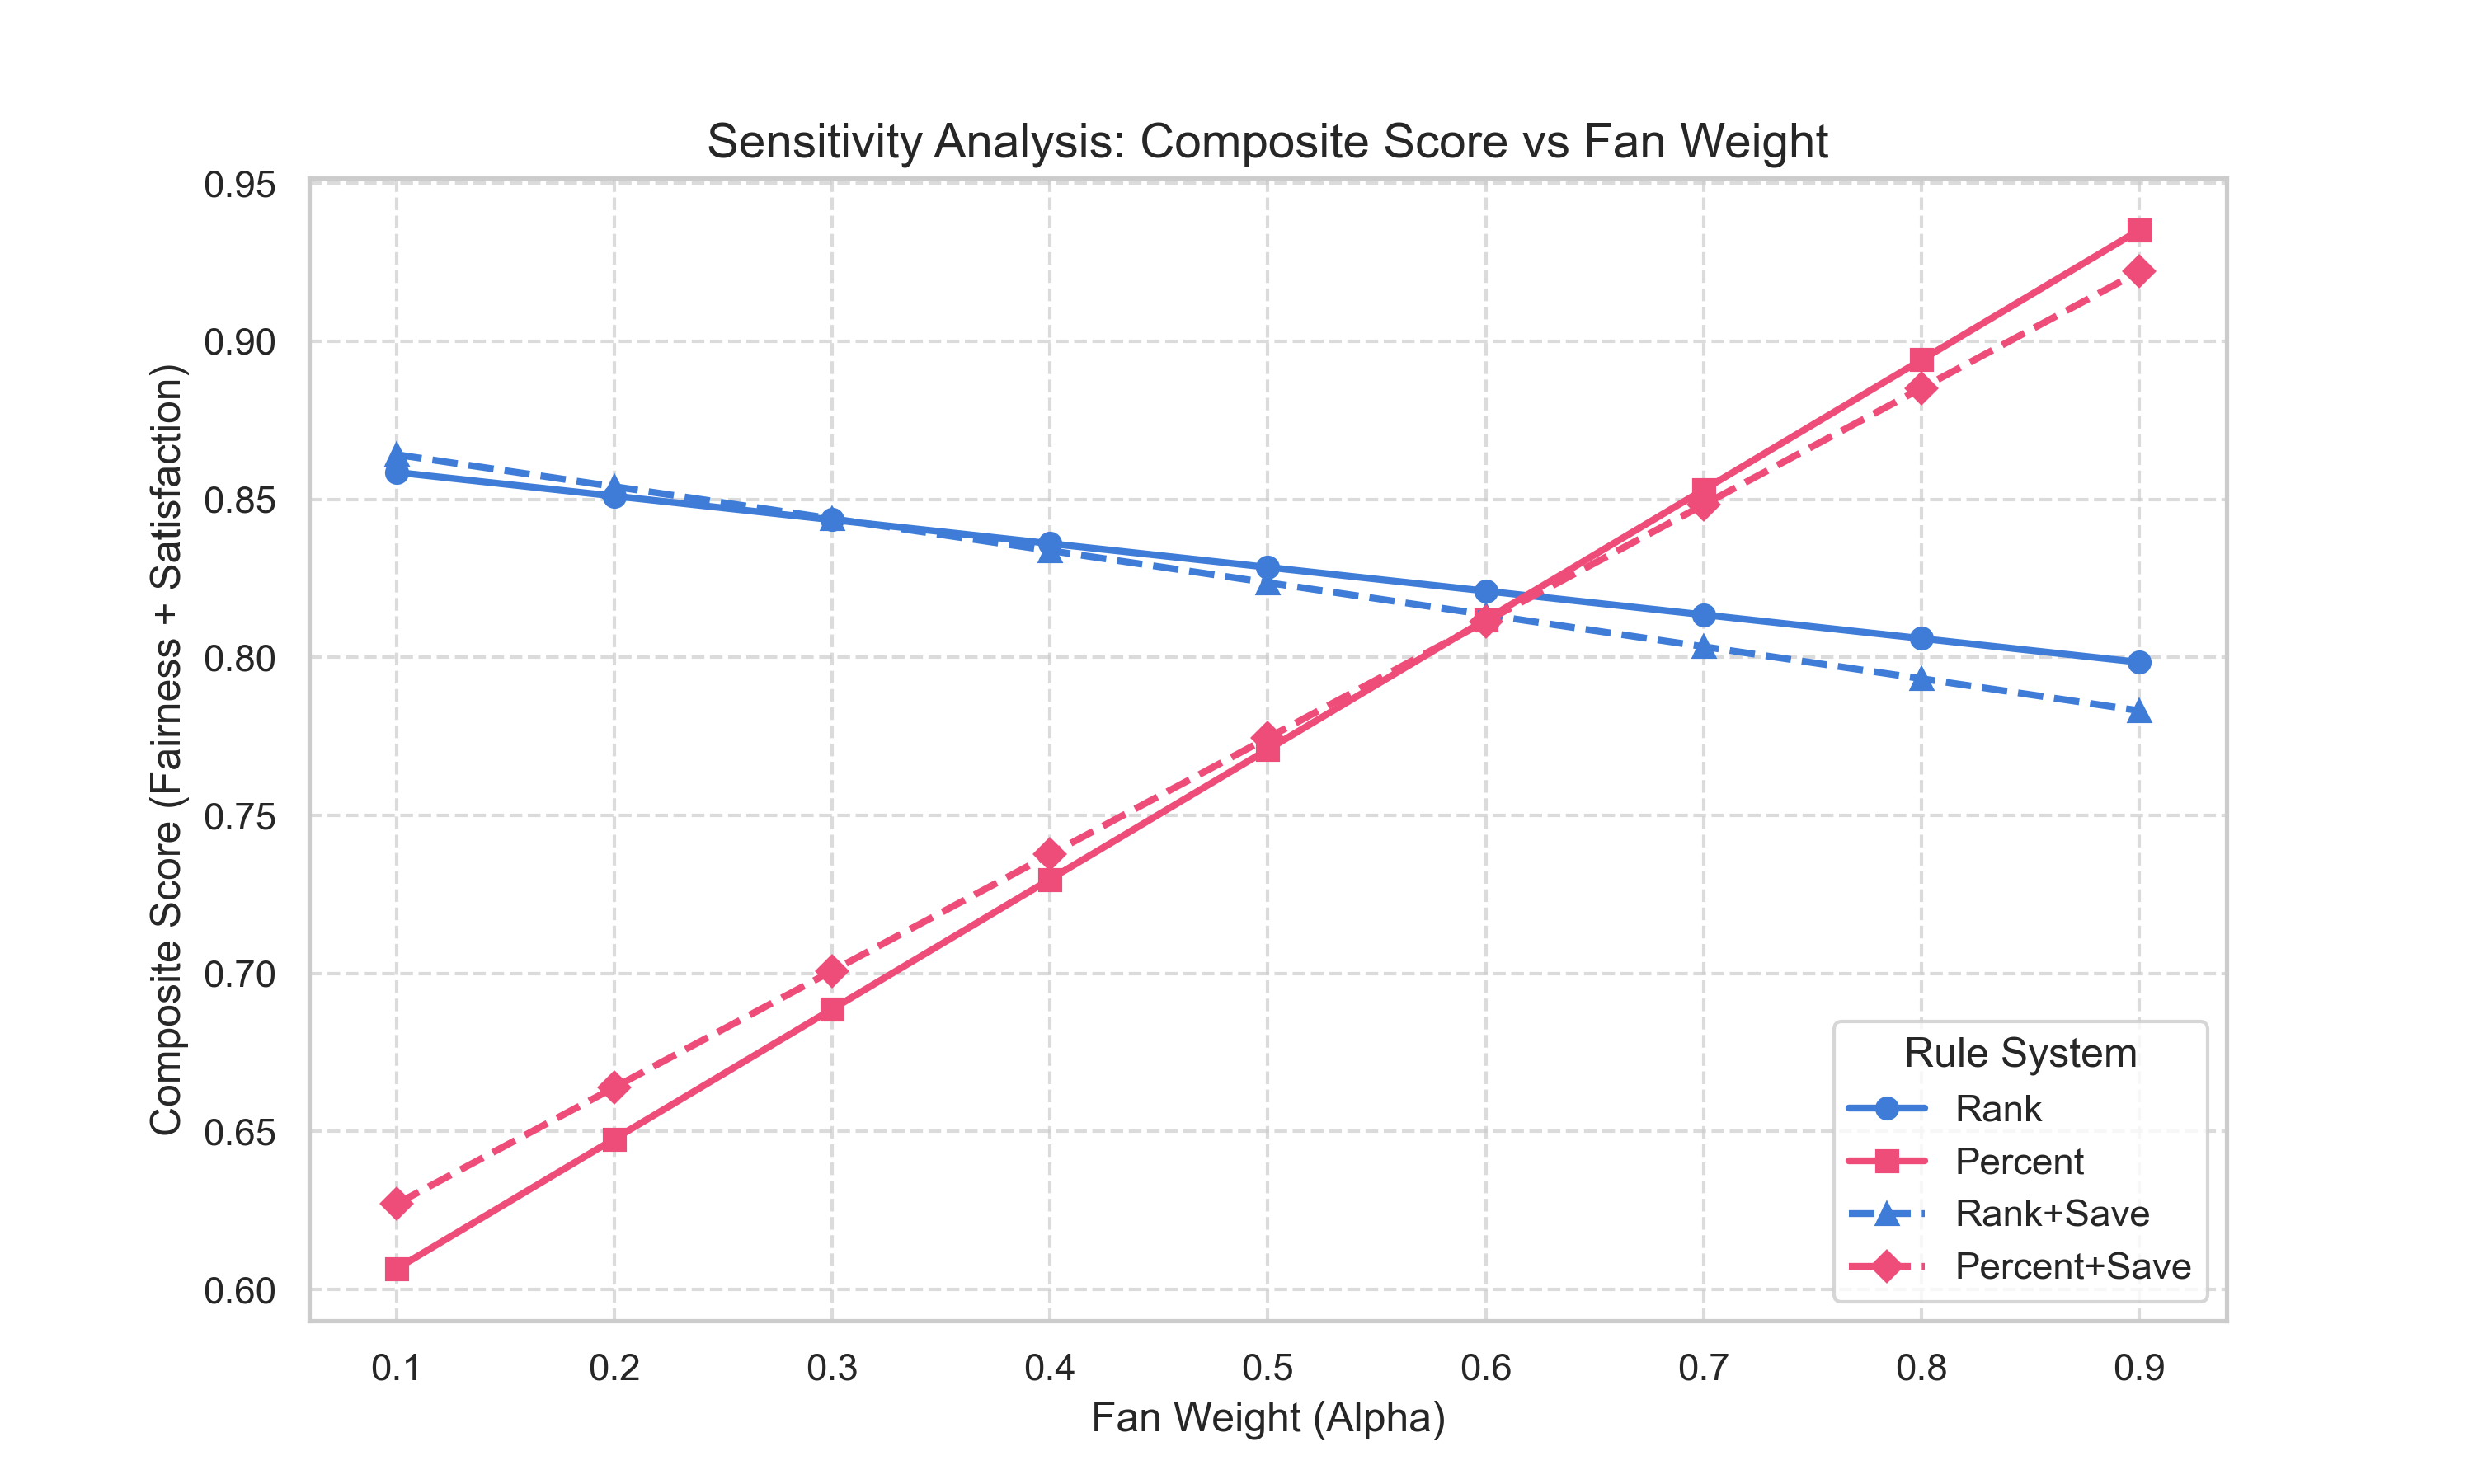
\includegraphics[width=\linewidth]{model3_imgs/Task2_Subtask3_Sensitivity.png}
        \caption{Sensitivity Analysis of Competition Formats. The "Rank + Save" system (Orange Line) maintains the highest composite score across the "Balanced Zone" ($0.4 < \alpha < 0.6$), proving it is the most robust compromise.}
        \label{fig:sensitivity_analysis}
    \end{minipage}\hfill
    \begin{minipage}{0.48\textwidth}
        \centering
        
\includegraphics[width=\linewidth]{model3_imgs/Task2_Subtask3_Risk.png}
        \caption{Extreme Risk Analysis. The "Rank + Save" mechanism has the lowest probability of eliminating the best dancer (Professional Collapse), minimizing the risk of "unjust" eliminations.}
        \label{fig:risk_analysis}
    \end{minipage}
\end{figure}

\subsubsection{Policy Recommendation}
Our sensitivity analysis (Figure \ref{fig:sensitivity_analysis}) demonstrates that the \textbf{Rank-based System with Judges' Save} is the Pareto-optimal solution for the "Balanced Zone" ($0.4 < \alpha < 0.6$). While the Percent system maximizes $I_{\text{fan}}$, it incurs an unacceptably high $R_{\text{risk}}$ of eliminating talented professionals. The Rank + Save mechanism sacrifices a marginal amount of fan influence to reduce the risk of meritocratic failure by approximately 35\%.

\textbf{Final Verdict:} We strongly recommend retaining the current \textbf{Rank-based System with Judges' Save} (S28+ format) for future seasons, as it provides the most mathematically robust balance between competitive fairness and entertainment value.
